
%%%%%%%%%%%%%%%%%%%%%%%%%%%%%%%%%%%%%%%%%%%%%%%%%%%%%%%%%%%%%%
%%%%%%%%%%%%%%%%% CANTILEVER BEAM DESIGN %%%%%%%%%%%%%%%%%%%%%%
%%%%%%%%%%%%%%%%%%%%%%%%%%%%%%%%%%%%%%%%%%%%%%%%%%%%%%%%%%%%%%%

\section{Cantilever Beam Design}
\label{cantilever}

This section describes the robust optimization of a cantilever beam.

\subsection{Problem Description}

 A cantilever beam of rectangular cross-section is subjected to a bending moment ${\cal{M}}~(N \cdot mm)$ and shear force ${\cal{V}}~(N)$. % as shown in Figure~\ref{fig}.
The bending stress in the beam is calculated as $\sigma=6{\cal{M}}/{bd^2}~(N/mm^2)$ and the average shear stress is calculated as ${\tau=3{\cal{V}}/2bd}~(N/mm^2)$, where $b$ is the width and $d$ is the depth of the beam. 
The maximum allowable stress in the form of bending, $\sigma_{allow}$, is $10~N/mm^2$ and the maximum allowable shear, $\tau_{allow}$, is $2~N/mm^2$.
The goal is to minimize the cross-sectional area $A~(mm^2)$ of the beam. The mathematical formulation of the problem is given below:
\beq \label{eq:beamdet}
\begin{aligned}
& \underset{b,d}{\text{minimize}}
& &  {{A}(b,d)=b d}, \\
& \text{subject to}
& & g_1(b,d,{\cal{M}}) = \frac{6{\cal{M}}{\F}}{bd^2\sigma_{allow}} - 1 \leq 0,\\
&&& g_2(b,d,{\cal{V}}) =\frac{3{\cal{V}}{\F}}{2bd\tau_{allow}} - 1 \leq 0,\\
&&& g_3(b,d) =\frac{d{\F}}{2b} - 1 \leq 0,\\
& \text{bounds}
& & 100~mm~\leq~b,d~\leq~600~mm,
\end{aligned}
\eeq
\noindent where the constraints $g_1$ and $g_2$ enforce bending and shear stress requirements, respectively, while $g_3$ imposes an aspect-ratio requirement for the rectangular cross-section. 
All the constraints are represented in standard normalized form. The design variables are the width and depth of the beam.


\subsection{Robust Optimization Problem}
The two allowable stresses ($\sigma_{allow}$ and $\tau_{allow}$) in Eq.~\eqref{eq:beamdet} are assumed to be precise (hence kept fixed) whereas the remaining parameters are assumed to have uncertainties and are therefor treated as random variables as listed in Table~\ref{tab:data_beam}. 
\begin{table}[h]
\caption[Data for cantilever beam design problem.]{Data and assumed uncertain parameters for cantilever beam design problem.}
\medskip
\centering 
\scalebox{0.95}{
  \begin{tabular}{cccccccc}
    \hline\hline
   Random   & Description    & Uncertainty        & $\tau_{min}$  & $\tau_{max}$   & Mean                & Standard   & Unit \\
   Variable   &     & Type        &   &    &                &   Deviation  & \\
    \hline\hline
    b                & Breadth        &    Epistemic       &  -10        &  10         & -                    &    -      &  $mm$   \\
    d                & Width          &    Epistemic       & -10         &  10         & -                    &     -     &  $mm$   \\
\hline
    $\cal{M}$                & Bending Moment &    Aleatory        &  -            &  -            &  $40\cdot 10^{6}$     &  40000    &  $N \cdot mm$   \\
    $\cal{V}$                & Shear Force    &    Aleatory        &  -            &  -            &  $150\cdot 10^{3}$    &   1500    &  $N$\\
\hline
\end{tabular}}
\label{tab:data_beam}
\end{table}
The bending moment and shear force are assumed to have normally distributed aleatory uncertainties with specified mean and standard deviations as shown in Table~\ref{tab:data_beam}. Only the constraints $g_1$ and $g_2$ which are functions of the bending moment and shear force are influenced by these aleatory variables. Unlike the three-bar truss problem where all random variables were also considered as design variables, the cantilever beam problem involves random variables which are not design variables, but their effects will be considered in the optimization procedure. The robust optimization problem can be written as:
\beq \label{eq:beamrob}
\begin{aligned}
& \underset{b,d}{\text{minimize}}
& &  {{A}(b,d)=\mu_{A}+\sigma_A^2}, \\
& \text{subject to}
& & g_1^r(b,d,{\cal{M}}) =\mu_{g_1} + k\sigma_{g_1} \leq 0,\\
&&& g_2^r(b,d,{\cal{V}}) =\mu_{g_2} + k\sigma_{g_2} \leq 0,\\
&&& g_3^r(b,d) =\mu_{g_3} + k\sigma_{g_3} \leq 0.
\end{aligned}
\eeq
In this problem only the epistemic random variables (width and depth) govern the cost function and the aspect-ratio constraint and therefore  the output standard deviations are unavailable for these functions: $\sigma_A$ and $\sigma_{g_3}=0$.
\paragraph{Surrogate Models:} The robust optimization results will be compared using both kriging and polynomial chaos. 
The kriging surrogate model is built with 20 training points and the polynomial chaos metamodel is a third order polynomial which is  also built with 20 training points.

\subsection{Optimization Results}


Table~\ref{tab:beamoptimum} presents the optimization results. It can be seen that the objective function value increases with the desired robustness, for example, the cross-sectional area increases by roughly $17\%$ for a design corresponding to $k=4$ compared to a deterministic design with no factor of safety. However, the robust design $(k=4)$ has $29\%$ less cross-sectional area (hence lighter) than a deterministic design with a factor of safety of 1.5.

\begin{table}[h!]
\caption{Optimization results for cantilever beam design problem.}
\medskip
\centering %m{0.15\textwidth}|m{0.35\textwidth}|m{0.35\textwidth}
\begin{tabular}{c| c c | c c| c| c}
\hline\hline
Type  & k  & $P_k$ &   Width  $b$  &  Depth $d$    & Area $A$     & No. of F/FG Evals. \\
{}    & {} & {}    & $mm$          & $mm$          & $\cdot 10^{3}$~$mm^2$        & $\&$ Iterations \\
\hline\hline
Initial Design & - & - & 300 & 300 & 90.0 & -  \\
\hline
Det $(F_s=1.0)$ & - & - & 335.5 & 335.4 & 112.5 & 33/33-7  \\
Det $(F_s=1.5)$ & - & - & 595.5 & 283.4 & 168.7 & 45/45-8  \\
\hline
Robust-KR & 0 & 0.5000 & 347.4 & 343.4 & 126.3 & 7046/3523-7  \\
Robust-PC & 0 & 0.5000 & 347.4 & 343.4 & 126.3 & 7917/7917-8  \\
\hline
Robust-KR & 1 & 0.8413 & 349.7 & 344.5 & 127.5 & 7146/3573-7  \\
Robust-PC & 1 & 0.8413 & 349.7 & 344.5 & 127.5 & 8037/8037-8  \\
\hline
Robust-KR & 2 & 0.9772 & 398.5 & 305.4 & 128.8 & 7686/3843-7  \\
Robust-PC & 2 & 0.9772 & 398.5 & 305.4 & 128.8 & 9661/9661-9  \\
\hline
Robust-KR & 3 & 0.9986 & 386.5 & 317.8 & 130.0 & 8694/4347-8    \\
Robust-PC & 3 & 0.9986 & 386.5 & 317.8 & 130.0 & 11669/11669-10 \\
\hline
Robust-KR & 4 & 0.9999 & 356.6 & 347.5 & 131.1 & 7286/3643-7  \\
Robust-PC & 4 & 0.9999 & 356.6 & 347.5 & 131.1 & 8196/8196-8  \\
\hline %0.9772/0.9986/0.9999
\end{tabular}
\label{tab:beamoptimum}
\end{table}



 \begin{figure}[h!]
  \centering
  \begin{minipage}[b]{0.75\linewidth}
    \includegraphics[width=1.0\textwidth]{BeamDesignSpace.eps} 
  \end{minipage}
\caption{Graphical solution to the minimum area beam design problem.}
\label{fig:beamdesignspace}
\end{figure}

Figure~\ref{fig:beamdesignspace} shows all three constraints plotted along with the objective function contours. The objective function is parallel to the constraint $g_2$, therefore, any point on the cure A--B is a feasible deterministic optimum. 
At point A, the constraints $g_2$ and $g_3$ are active; at point B, the constraints $g_1$ and $g_2$ are active; while any point on the curve A--B has the constraint $g_2$ active. 
Through robust optimization, the optimum solution is moved by a distance of $k$ standard deviations away from the deterministic solution, which is shown by an increment in the objective function values in Table~\ref{tab:beamoptimum}. 
However, the robust optimization accounts for the exact amount of uncertainty in the problem and achieves a reduced cost function compared to deterministic designs employing an arbitrary factor of safety which could easily be over-conservative or under-conservative.



\subsubsection{Simulation Requirements}

\begin{figure}[h!]
  \centering
  \begin{minipage}[b]{0.8\linewidth}
    \includegraphics[width=1.0\textwidth]{beamiterhist.eps}
  \end{minipage}
\caption{Optimization history for the beam design problem.}
\label{fig:beamiterhist}
\end{figure}

The box-constrained optimizations took only 2 to 3 function and gradient evaluations to reach the extremum. On average the robust optimization takes about 7500 function and gradient evaluations (includes the constraint evaluations), when compared to the deterministic optimization whose simulation needs are many folds lesser. Simulation requirements for the polynomial chaos method 
is roughly $20\%$ higher than that of kriging.

Figure~\ref{fig:beamiterhist} plots the change in the objective function with the number of optimization iterations for different tested cases (deterministic and robust). 


\subsubsection{Output PDF and CDF}
Figure~\ref{fig:beamcon1} shows the probability density and cumulative distribution functions of constraints $g_1$ and $g_2$. 
The PDFs show the spread of possible values taken by the constraints corresponding to different robust designs, whereas the CDFs show the probability of obtaining a specified value or less.  
Knowing the spread of values helps a designer to make informed decisions about the performance of the design. For example, a robust design corresponding to $k=4$ (red lines) features negligible occurrence of $g_i>0$ (signifies a constraint violation). It can also be observed that the constraint values are normally distributed.
\begin{figure}[H]
  \centering
  \begin{minipage}[b]{0.48\linewidth}
    \includegraphics[width=1.0\textwidth]{beampdfallcon1.eps} \subcaption{PDF $(g_1)$}
  \end{minipage}
  \begin{minipage}[b]{0.48\linewidth}
    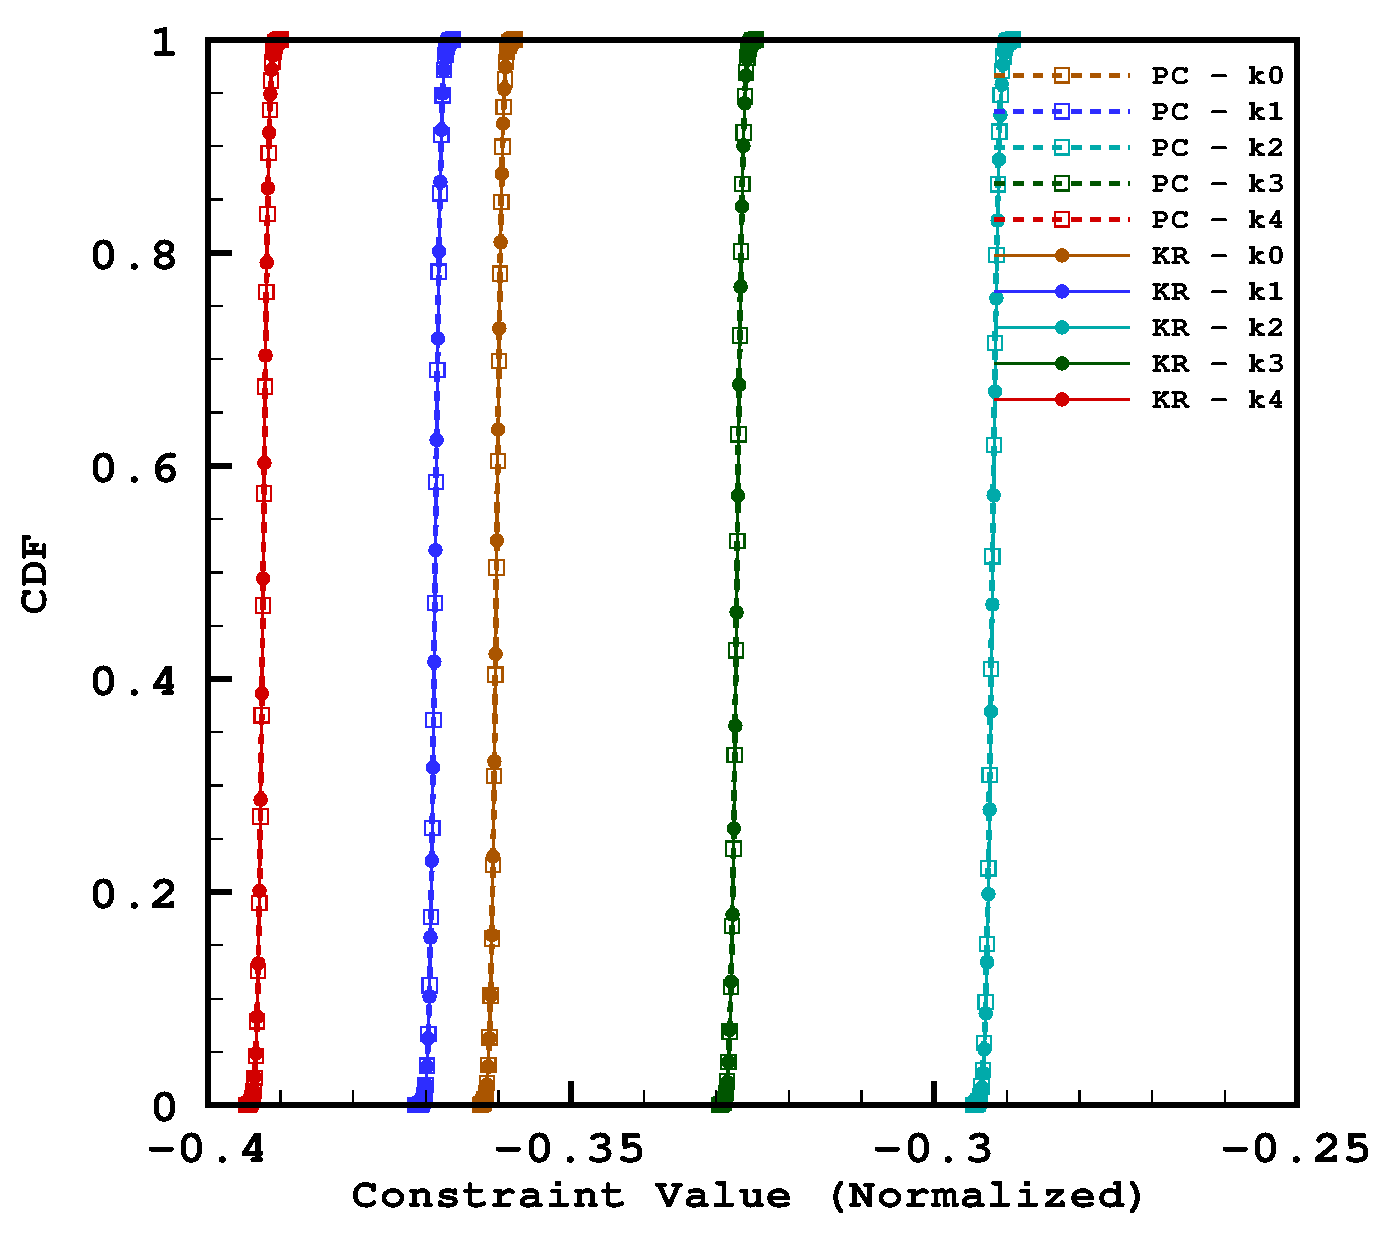
\includegraphics[width=1.0\textwidth]{beamcdfallcon1.eps} \subcaption{CDF $(g_1)$} 
  \end{minipage}
  \begin{minipage}[b]{0.48\linewidth}
    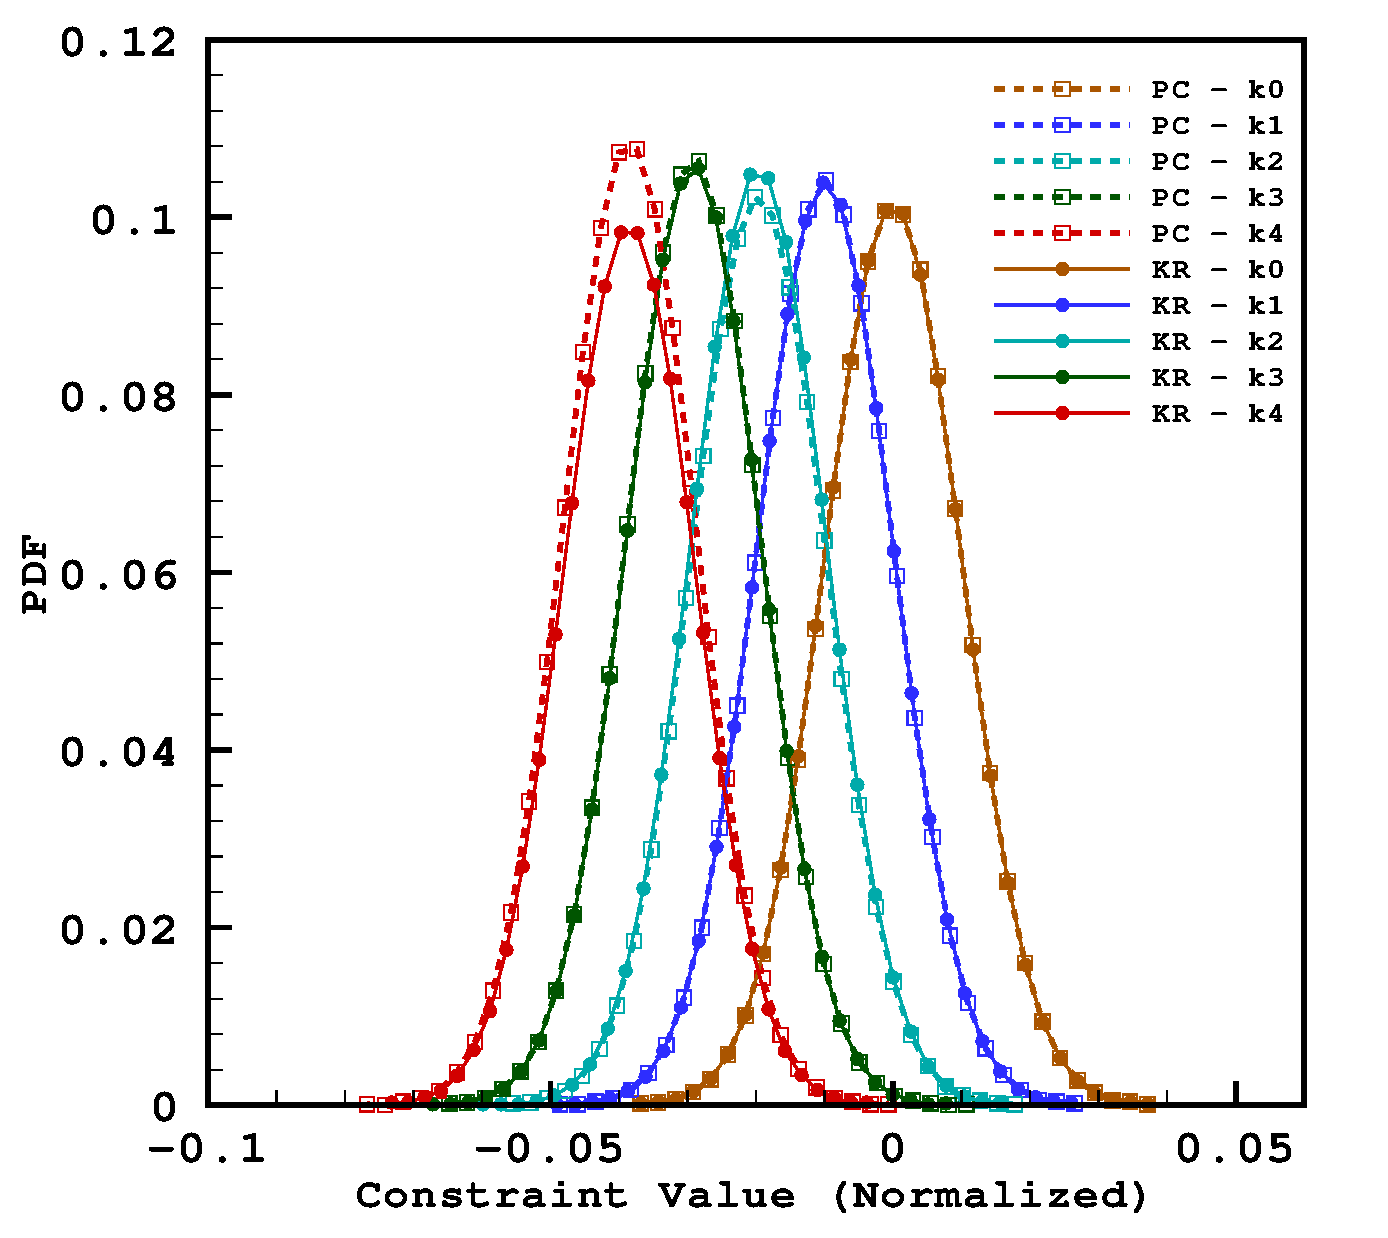
\includegraphics[width=1.0\textwidth]{beampdfallcon2.eps} \subcaption{PDF $(g_2)$}
  \end{minipage}
  \begin{minipage}[b]{0.48\linewidth}
    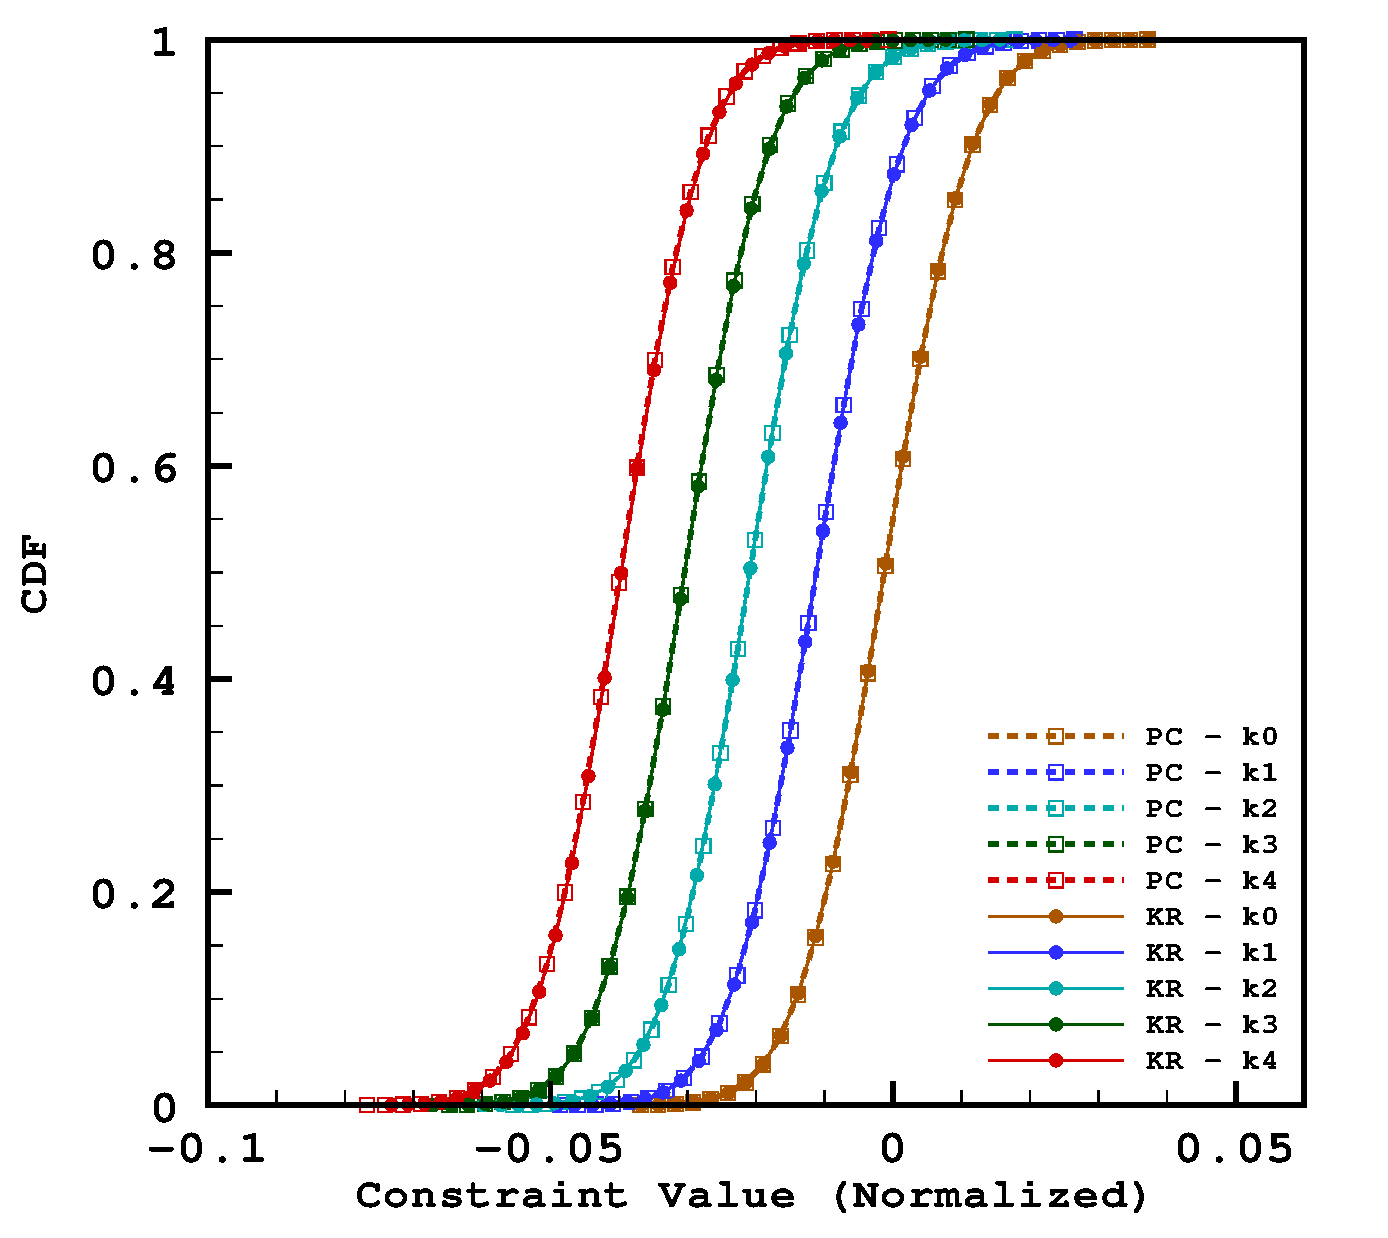
\includegraphics[width=1.0\textwidth]{beamcdfallcon2.eps} \subcaption{CDF $(g_2)$} 
  \end{minipage}
\caption{Output PDF (left) and CDF (right) of constraint $g_1$ and $g_2$.}
\label{fig:beamcon1}
\end{figure}
\clearpage
